\chapter{Grant Cardone: Audience, Scale, and Asset Control}

This chapter follows the School of Hard Knocks interview with Grant Cardone, curated for Video2Book by LazyingArt LLC. The useful mathematics here is not blackboard mathematics; it is commercial arithmetic: scale, ratios, unit counts, funnel conversion, monthly drawdown, and the difference between income that stops and assets that keep producing. We will keep Cardone's order of attack. He begins with audience before institutions, turns to boredom and urgency, breaks the spell of a million dollars with a division problem, and then builds toward people, brand, real estate, scale, closing, and the final question of what money is for.

\section{Audience Before Institutions}

Cardone opens with a claim about capital formation. He says that his group has raised \(\$1.1\) billion through crowdfunding on the internet. The contrast is important: he does not describe the mechanism as asking Mark Cuban, Blackstone, or a small circle of wealthy institutions for money. He describes it as building a large audience, making offers to that audience, and asking whether they want to invest.

That gives us the first working model of the chapter. Money is not merely a static quantity in a bank account. It moves through a channel:

\[
\hbox{audience}+\hbox{trust}+\hbox{offer} \longrightarrow \hbox{capital}.
\]

This is not a theorem. It is the operating claim that organizes the interview. The audience is the asset-like object that can be activated repeatedly. The offer is the test of whether the audience is only watching or is willing to act.

\begin{definition}
In these notes an \emph{audience} means the accumulated set of people who know, watch, buy from, or may invest with the entrepreneur. It is not yet capital, but it is a possible path to capital.
\end{definition}

Cardone immediately widens the reference frame. He compares himself not with the person next to him, but with the amount of money he says is circulating: roughly \(\$80\) trillion in U.S. dollars. The numerical claim should be treated as his stated frame, not as an independently verified monetary aggregate. The function of the number in the interview is to change the scale of the listener's imagination.

\begin{equation}
M_{\mathrm{USD}} \approx \$80\text{ trillion}.
\end{equation}

The point is not that this whole stock is available to any one person. The point is that Cardone wants the listener to stop treating a small local comparison group as the universe of possible money.

\section{Boredom, Urgency, and the Cost of Free Time}

The first formal question is about self-improvement. The interviewer asks about free time, cheap entertainment, distraction, and getting serious. Cardone's answer is deliberately abrasive, but the mechanism is simple enough to state cleanly: boredom changes the environment in which decisions are made.

He does not begin with a productivity system. He begins with a danger model. Free time becomes boredom; boredom lowers the threshold for bad company, bad places, and bad habits; those conditions produce decisions that destroy momentum. The positive alternative is urgency: a schedule full enough that there is less room for drift.

\begin{figure}
\centering
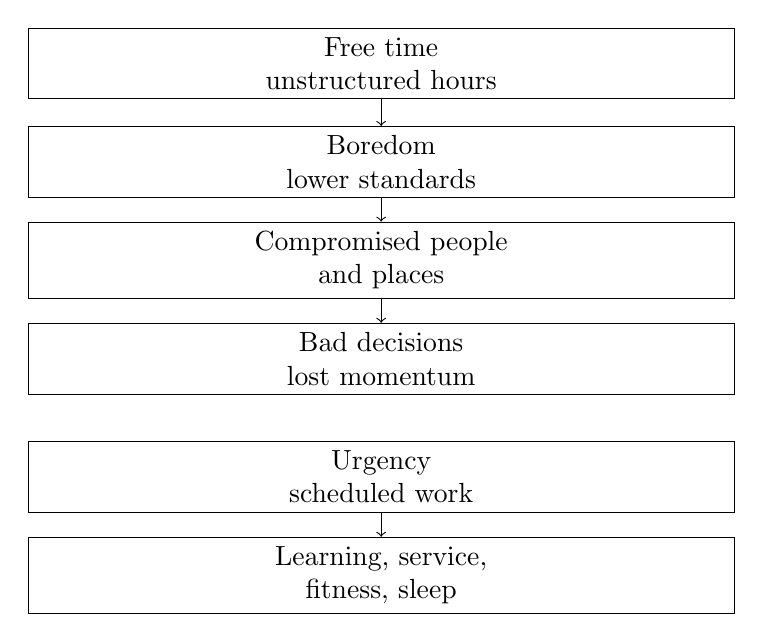
\begin{tikzpicture}
\node[draw, align=center, text width=.72\linewidth] (a) at (0,0) {Free time\\unstructured hours};
\node[draw, align=center, text width=.72\linewidth] (b) at (0,-1.25) {Boredom\\lower standards};
\node[draw, align=center, text width=.72\linewidth] (c) at (0,-2.5) {Compromised people\\and places};
\node[draw, align=center, text width=.72\linewidth] (d) at (0,-3.75) {Bad decisions\\lost momentum};
\node[draw, align=center, text width=.72\linewidth] (e) at (0,-5.25) {Urgency\\scheduled work};
\node[draw, align=center, text width=.72\linewidth] (f) at (0,-6.5) {Learning, service,\\fitness, sleep};
\draw[->] (a) -- (b);
\draw[->] (b) -- (c);
\draw[->] (c) -- (d);
\draw[->] (e) -- (f);
\end{tikzpicture}
\caption{The interview's first operating diagram: unstructured free time is treated as a risk path, while urgency is treated as a stabilizing path.}
\end{figure}

This is also where he introduces the million-to-billion shock. A billion is not reached by making one million once. The bare arithmetic is already large:

\begin{equation}
\$1{,}000{,}000{,}000=1{,}000\times \$1{,}000{,}000.
\end{equation}

But Cardone's point is that the bare identity understates the practical burden. A person does not keep every dollar made. Taxes, payroll, retained margin, mistakes, and losses mean the number of million-dollar wins required to keep a billion is greater than \(1{,}000\).

\subsection{Question \& Answer}

\paragraph{Question.} Why does free time become a business risk rather than simply a reward?

\paragraph{Answer.} In Cardone's account, free time is risky because it creates an empty decision environment. The risk is not idleness alone; it is the sequence from idleness to boredom, from boredom to compromised surroundings, and from compromised surroundings to decisions that make the next day weaker. Urgency, in this framework, is not merely emotional intensity. It is a schedule design that protects the person from drift.

\section{The Million-Dollar Calculation}

The next question asks about the mindset shift around money. Cardone answers by attacking one of the most common symbols of financial success: the million dollars. He asks the interviewer his age, assumes he is \(21\), asks how long he wants to live, accepts \(80\), and then divides.

The calculation is the cleanest worked example in the interview. Assume no new income and no inflation. Then the million dollars must be spread over \(80-21=59\) years.

\begin{align}
\hbox{remaining years} &= 80-21=59,\\
\hbox{remaining months} &= 59\times 12=708,\\
\hbox{monthly draw} &= \frac{\$1{,}000{,}000}{708}
\approx \$1{,}412.
\end{align}

Cardone rounds this to about \(\$1{,}400\) per month. The mathematical point is not subtle, but it is effective. A million dollars as a headline number and a million dollars as a lifetime spending stream are different objects.

\subsection{Question \& Answer}

\paragraph{Question.} Why does the same \(\$1{,}000{,}000\) feel large in one frame and small in another?

\paragraph{Answer.} Because the frame changes from stock to flow. As a stock, \(\$1{,}000{,}000\) sounds like a large pile. As a flow over \(708\) months, it becomes roughly \(\$1{,}400\) per month before inflation, emergencies, taxes, or mistakes. Cardone's point is that the listener should not confuse a round number with freedom.

He then makes a sharper social claim: people learn what counts as a lot of money from people who may not have much of it. We do not have to adopt every rhetorical edge of that claim to preserve its function. It is a warning about reference points. If the target is too small, reaching it may produce disappointment rather than freedom.

\section{From Poor to Rich to Wealthy}

The interview then moves from the size of money to the structure of money. The interviewer invokes the familiar phrase that the poor get poorer and the rich get richer. Cardone interrupts the frame: rich is not wealthy.

The distinction is central. Rich, in his usage, can mean high income, a large house, a country club life, a good salary, and visible comfort. Wealthy means something else: a durable structure that continues when the person stops working.

\begin{equation}
\hbox{poor}\longrightarrow \hbox{middle class}\longrightarrow \hbox{rich}\longrightarrow \hbox{wealthy}.
\end{equation}

This arrow is a conceptual progression, not a law. The danger in the middle is comfort. The danger in the rich stage is dependence on the current income producer. Cardone uses his father's death as the concrete case. His father died at \(52\), and Cardone says that within about \(72\) hours the family's situation changed because income, decision-making, and the household's economic engine stopped.

\begin{definition}
In this chapter, \emph{rich} means high visible income or comfort that may still depend on the current earner. \emph{Wealthy} means ownership, brand, assets, or institutions that can continue beyond the earner's immediate labor.
\end{definition}

He also invokes Sam Walton as a contrast: a founder dies, but the enterprise and ownership continue. The claim is not simply that wealth is more money than rich. The claim is that wealth has a different time structure. It survives.

\begin{remark}
Estate taxes, inheritance, and family ownership are mentioned in the interview as mechanisms by which money can either dissipate or continue. The transcript does not support a technical tax analysis, so the notes should keep the point structural: stopped income is fragile; durable ownership is less fragile.
\end{remark}

\section{Go to Zero, Then Build Through People}

The question about the best financial advice becomes a story from \emph{Undercover Billionaire}. Cardone says he was given \(\$100\) and asked to build a business, with a personal target of \(\$10\) million in \(90\) days and without using his name. He treats this as a puzzle.

\begin{equation}
\$100 \longrightarrow \$10{,}000{,}000,
\qquad
\frac{10{,}000{,}000}{100}=100{,}000.
\end{equation}

The obvious instinct is to preserve and manage the \(\$100\). Cardone's answer is the opposite: return it, go to zero, and stop thinking like a manager of a tiny amount of capital. In the interview this is a provocative rule, not a universal personal-finance doctrine. The mechanism he wants to isolate is that small money can produce defensive behavior, while people and reinvestment can create scale.

\subsection{Question \& Answer}

\paragraph{Question.} Why would someone return the only \(\$100\) he has?

\paragraph{Answer.} In Cardone's story, keeping the \(\$100\) makes the problem too small. It tempts him to manage scarcity. Returning it forces a different search: Who can I meet? What relationship can I create? What offer can I make? What can be reinvested into skill, marketing, brand, information, speed, and confidence? The claim is not that cash is useless. The claim is that the path from \(\$100\) to \(\$10\) million cannot be explained by guarding the original \(\$100\).

This leads naturally to the next object: people. Earlier, Cardone demonstrates the idea with the interviewer's credit card. Money does not travel to us in the abstract; it comes through another human being. The ethical path is not theft, which can happen only once and destroys trust. The repeatable path is relationship.

\[
\hbox{people}\longrightarrow \hbox{trust}\longrightarrow \hbox{offer}\longrightarrow \hbox{money}.
\]

The brand question follows immediately. Cardone's answer is not elegant branding theory. It is persistence: show up, be known, tolerate ridicule, and become difficult to ignore. His rough anecdote about a man who kept showing up for fights is not advice to fight; it is an analogy about repeated presence. In the business version, the repeated act is not violence. It is visibility, work, and offers.

\section{Real Estate, Scale, and Asset-Backed Lending}

The interviewer then asks about Cardone's first real estate deals and suggests a jump from one unit to \(38\) units. Cardone corrects the sequence. First came a single-family house. Twenty-eight days later came another single-family house. Three years later came \(48\) units. The correction matters because the lesson is not overnight enlargement. It is learning from a bottleneck.

The bottleneck has a name in the story: Janet. She rents the single-family house. When she moves out, the rent from that house goes to zero.

\begin{equation}
1\hbox{ tenant leaves }1\hbox{ unit}
\quad \Longrightarrow \quad
\$0\hbox{ rent from that asset}.
\end{equation}

This is one-unit fragility. It is not merely that the property is small. It is that the income stream depends on one occupant. Cardone's solution is not to improve the slogan around single-family rentals. His solution is to stop buying one unit.

For a \(48\)-unit property, he gives a simple income example. If each unit produces \(\$1{,}000\) per month, then gross monthly rent is

\begin{equation}
48\times \$1{,}000=\$48{,}000\hbox{ per month}.
\end{equation}

\begin{figure}
\centering
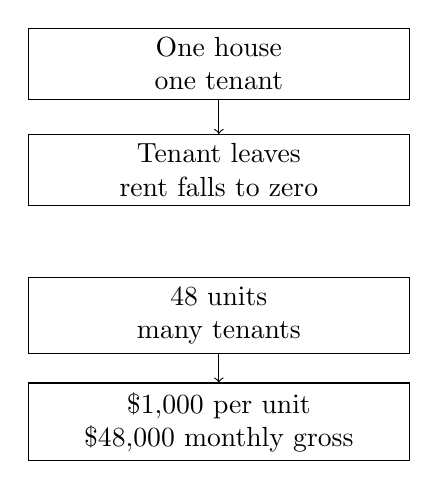
\begin{tikzpicture}
\node[draw, align=center, text width=.38\linewidth] (one) at (0,0) {One house\\one tenant};
\node[draw, align=center, text width=.38\linewidth] (zero) at (0,-1.35) {Tenant leaves\\rent falls to zero};
\node[draw, align=center, text width=.38\linewidth] (many) at (0,-3.2) {48 units\\many tenants};
\node[draw, align=center, text width=.38\linewidth] (income) at (0,-4.55) {\(\$1{,}000\) per unit\\\(\$48{,}000\) monthly gross};
\draw[->] (one) -- (zero);
\draw[->] (many) -- (income);
\end{tikzpicture}
\caption{Cardone's rental lesson: one-unit income is fragile, while many-unit income can be underwritten as an asset stream.}
\end{figure}

The stated deal numbers are also part of the mathematical spine. Cardone says he raised or put in \(\$350{,}000\), signed a \(\$1.9\) million note, and made \(\$3.7\) million net on the deal.

\begin{align}
\hbox{capital raised or invested} &\approx \$350{,}000,\\
\hbox{note} &\approx \$1.9\text{ million},\\
\hbox{claimed net profit} &\approx \$3.7\text{ million}.
\end{align}

Then comes the mental extrapolation:

\begin{equation}
10\times \$3.7\text{ million}=\$37\text{ million}.
\end{equation}

The point is not that ten identical deals were guaranteed. The point is that one scalable deal changed the unit of imagination. Before this, the single-family houses had some cash flow. After this, one transaction suggested a path to tens of millions.

The lending point is equally important. Cardone says the bank did not lend to ``Grant'' in the ordinary personal-credit sense. It lent to the LLC or the apartment complex. We should not add loan covenants or nonrecourse details that are not in the transcript. The supported mechanism is narrower: the income-producing entity changes the underwriting conversation.

\[
\hbox{asset income}+\hbox{entity structure}
\longrightarrow
\hbox{loan considered against the property}.
\]

\section{Follow the Money, Funnels, and Closing by Serving}

The late middle of the interview broadens the scale lesson. Cardone argues that if a company is too small, the owner is controlled by a few employees or a few customers. His examples are deliberately blunt: three employees create dependency; thirty still may not be enough; three thousand means the owner no longer personally carries every employee problem.

The same pattern appears in customers. If there are too few, each customer can push the company around. Scale creates optionality. The principle can be written as a dependency ratio:

\[
\hbox{fragility}\sim \frac{1}{\hbox{number of independent customers, employees, or units}}.
\]

This is not a formal law of business. It is a compact way of recording the mechanism in the interview: dependence on one person, one tenant, one buyer, or one employee is dangerous.

Cardone then tells the yacht story. He sees clusters of very large boats and concludes that the best place to anchor is where the money already is. The story is not really about boats. It is about using observed concentration as information. He calls this ``follow the money.''

After a production interruption in the source video, the interview returns to scale, talent, and sales. Cardone says success attracts success: a successful team can recruit better players, a successful event can attract better speakers, and a larger enterprise can retain better people.

The sales section returns to the opening claim. He says \(80\%\) of what his organization does is free, and the paying \(20\%\) produces very large revenue. He also gives a more specific funnel: \(16\) million online people, \(154{,}000\) buyers of products or services, \(450{,}000\) people who raised their hands as interested investors, \(13{,}000\) actual investors, and \(\$1.1\) billion raised.

\begin{figure}
\centering
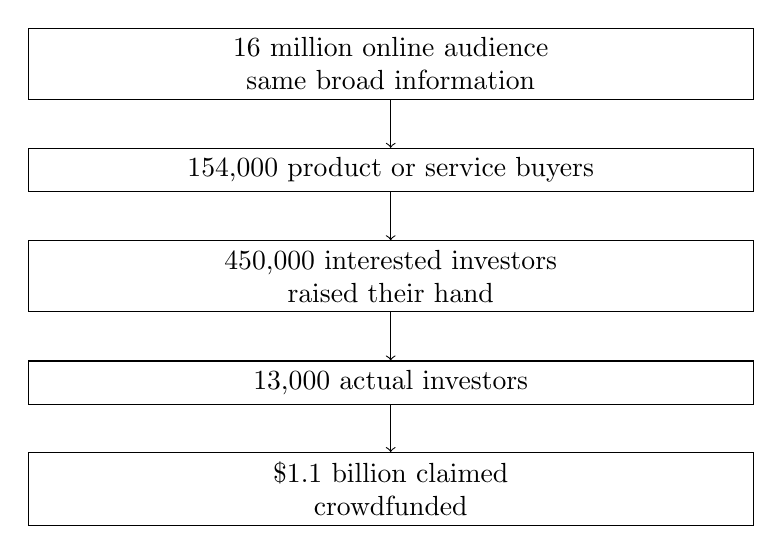
\begin{tikzpicture}
\node[draw, align=center, text width=.74\linewidth] (a) at (0,0) {16 million online audience\\same broad information};
\node[draw, align=center, text width=.74\linewidth] (b) at (0,-1.35) {154,000 product or service buyers};
\node[draw, align=center, text width=.74\linewidth] (c) at (0,-2.7) {450,000 interested investors\\raised their hand};
\node[draw, align=center, text width=.74\linewidth] (d) at (0,-4.05) {13,000 actual investors};
\node[draw, align=center, text width=.74\linewidth] (e) at (0,-5.4) {\(\$1.1\) billion claimed\\crowdfunded};
\draw[->] (a) -- (b);
\draw[->] (b) -- (c);
\draw[->] (c) -- (d);
\draw[->] (d) -- (e);
\end{tikzpicture}
\caption{A transcript-grounded funnel. The exact business categories overlap in the telling, but the intended mechanism is clear: broad free attention narrows into buyers, investors, and capital.}
\end{figure}

Here the arithmetic must be handled carefully. Cardone speaks the investor conversion quickly and inconsistently. The calculation is

\begin{equation}
\frac{13{,}000}{450{,}000}
\approx 0.0289
=2.89\%.
\end{equation}

So the supported figure is roughly \(2.9\%\), not \(0.28\%\). His spoken ``2.8\%'' is close; the ``0.28\%'' line is not.

For product buyers, the transcript gives another useful ratio:

\begin{equation}
\frac{154{,}000}{16{,}000{,}000}
\approx 0.0096
=0.96\%.
\end{equation}

That is approximately \(1\%\), though the transcript describes it as less than one tenth of one percent. The chapter should preserve the funnel while being honest about the arithmetic.

Repeat purchases matter because Cardone reframes closing. He says closing is not the moment when the seller traps the buyer; it is the moment when the buyer can finally be served. He claims \(45{,}000\) of \(154{,}000\) buyers purchased three, four, five, six, seven, or eight things. The ratio is

\begin{equation}
\frac{45{,}000}{154{,}000}
\approx 0.292
=29.2\%.
\end{equation}

That supports his spoken ``like \(30\%\)'' point. In the logic of the interview, the first close is not the end of the relationship. It is the beginning of service and repeat trust.

\section{Summary: Production, Discipline, and What Money Is For}

The closing turn is personal. The interviewer asks about the turning point in Cardone's life: baseball not working out, drugs, the wrong crowd, and getting his life on track. Cardone answers that it took ten years to lose and about three years to clean up the damage. He changed friends, changed places, made amends, showed up early, stayed late, and turned free time into work, learning, service, or sleep.

This ending sends us back to the beginning. Boredom was the first danger in the interview, and boredom returns as the continuing danger. Cardone says he still avoids late-night settings that would be bad for him. He says he manufactures dissatisfaction rather than waiting for a bottom. In the language of the chapter, he is designing an operating environment.

The final claim is about the use of money. Cardone argues that money matters because real obligations require it: family, schools, hospitals, churches, businesses, employees, and assets. Good feelings do not buy groceries. The point is stated roughly in the interview, but the structure is clear:

\[
\hbox{production}
\longrightarrow
\hbox{income}
\longrightarrow
\hbox{reinvestment}
\longrightarrow
\hbox{assets}
\longrightarrow
\hbox{durable capacity to help and choose}.
\]

The chapter's mathematical payload is therefore compact. A million dollars becomes \(\$1{,}400\) a month when divided over a young lifetime. One tenant leaving one house can make the rent zero. Forty-eight units at \(\$1{,}000\) per month produce \(\$48{,}000\) in gross monthly rent. \(\$3.7\) million repeated ten times becomes \(\$37\) million. \(13{,}000\) investors out of \(450{,}000\) interested people is about \(2.9\%\). \(45{,}000\) repeat buyers out of \(154{,}000\) buyers is about \(29.2\%\).

The interview's doctrine can be summarized in one sentence: stop treating money as a symbol, and start treating it as a flow through people, offers, trust, scale, entities, and assets.